\section{Kvantmekanik}

\paragraph{Brister i klassisk fysik}
Redan innan kvantmekaniken formulerades, fanns det brister i det experimentella beviset för den klassiska fysiken.

\subparagraph{Ultravioletta katastrofen}
Ett bevis var att den klassiska förutsägelsen av svartkroppsstrålning var
\begin{align*}
	I(\nu, T) = \frac{2kT\nu^{2}}{c^{2}},
\end{align*}
som divergerar för stora frekvenser. Observationer av svartkroppsstrålning var naturligtvis inte i närheten av detta utan gick mot $0$ även för höga frekvenser.

Max Planck sägs att ha upptäckt kvantmekaniken vid att härleda intensitetsfördelningen för svartkroppsstrålning under antagandet att energinivåerna i kroppen var diskreta kvanta av $h\nu$, där $h$ är den nu införda Plancks konstant. Han fick
\begin{align*}
	I(\nu, T) = \frac{2h\nu^{3}}{c^{2}}\frac{1}{e^{\frac{h\nu}{kT}} - 1}.
\end{align*}
Denna går både mot $0$ för höga frekvenser och beter sig som den klassiska förutsägelsen vid  låga frekvenser. Einstein gissade senare att $h\nu$ var energien för partiklarna som bygger upp ljus - fotoner.

\subparagraph{Fotoelektriska effekten}
Om man bestrålar metaller med elektromagnetisk strålning, frigörs elektroner (upptäckta vid det här laget) från metallet. Man kunne sätta metallet i närheten av en anod så att en spänningsskillnad mellan metallet och anoden kunde attrahera metaller till anoden. Vid at elektrisk koppla de två samman, kunde man mäta strömmen som orsakades av de frigjorda elektronerna. Det som observerades var:
\begin{itemize}
	\item Det frigjordes bara elektroner om den inkommande strålningen hade en frekvens över en viss gränsfrekvens.
	\item Under denna gränsfrekvensen spelade strålningsintensiteten ingen roll.
	\item Över gränsfrekvensen mättes den maximala elektronenergin som $E = h\nu - W$.
\end{itemize}

Detta var svårt att förklara med klassisk fysik.

\subparagraph{Comptonspridning}
Elektromagnetisk strålning kan spridas på elektroner. Klassiskt är det svårt att förklara spridningsmönstret som uppstår, eftersom elektromagnetisk strålning är vågor. Däremot kan man anta att strålningen består av fotoner med rörelsemängd och energi enligt speciell relativitetsteori och resultaten från fotoelektriska effekten, som illustrerad i figur \ref{fig:compton_collision}.

\begin{figure}[!ht]
	\centering
	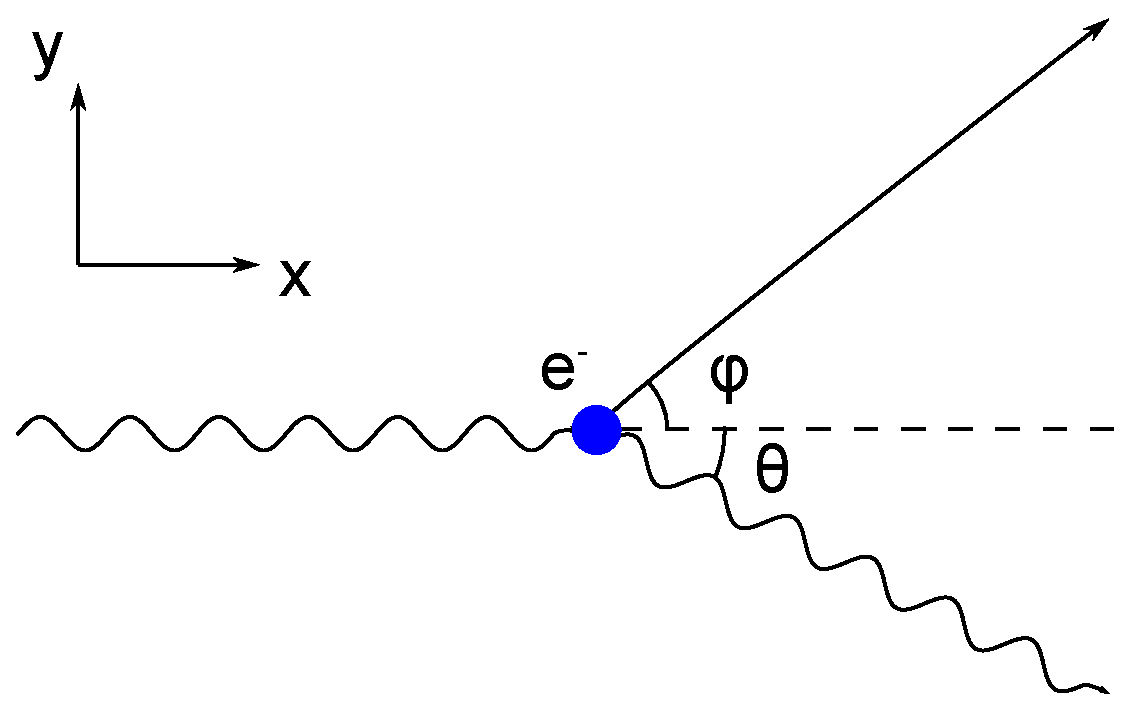
\includegraphics[width = 0.5\textwidth]{./Images/compton_collision.eps}
	\caption{Illustration av studs mellan en foton och en elektron.}
	\label{fig:compton_collision}
\end{figure}

Energins bevarande ger
\begin{align*}
	h\nu + m_{e, 0}c^{2} = E_{e} + h\nu'
\end{align*}
och rörelsemängdens bevarande ger
\begin{align*}
	h\frac{\nu}{c} = h\frac{\nu'}{c}\cos{\phi} + p_{e}'\cos{\theta}, \\
	h\frac{\nu'}{c}\sin{\phi} - p_{e}'\sin{\theta} = 0.
\end{align*}
Vi omformulerar förste rörelsemängdekvationen till
\begin{align*}
	h\frac{\nu}{c} - h\frac{\nu'}{c}\cos{\phi} = p_{e}'\cos{\theta}
\end{align*}
och kvadrerar för att få
\begin{align*}
	h^{2}\frac{\nu^{2}}{c^{2}} - 2h^{2}\frac{\nu\nu'}{c^{2}}\cos{\phi} + h^{2}\frac{\nu'^{2}}{c^{2}}\cos^{2}{\phi} = p_{e}'^{2}\cos^{2}{\theta}.
\end{align*}
Kombinerat med kvadratet av den andra rörelsemängdsekvationen ger detta
\begin{align*}
	h^{2}\frac{\nu^{2}}{c^{2}} + h^{2}\frac{\nu'^{2}}{c^{2}} - 2h^{2}\frac{\nu\nu'}{c^{2}}\cos{\phi} = p_{e}'^{2}.
\end{align*}
Energins bevarande ger vidare
\begin{align*}
	E_{e} = h\nu - h\nu' + m_{e, 0}c^{2}.
\end{align*}
Vi kvadrerar och kombinerar med massa-energi-sambandet från speciell relativitet och får
\begin{align*}
	h^{2}(\nu - \nu')^{2} + 2h(\nu - \nu')m_{e, 0}c^{2} + m_{e, 0}^{2}c^{4} &= p_{e}'^{2}c^{2} + m_{e, 0}^{2}c^{4} \\
	                                                                        &= h^{2}\nu^{2} + h^{2}\nu'^{2} - 2h^{2}\nu\nu'\cos{\phi} + m_{e, 0}^{2}c^{4}, \\
	(\nu - \nu')m_{e, 0}c^{2}                                               &= h\nu\nu'(1 - \cos{\phi}).
\end{align*}
Vi skriver nu om till våglängd och får
\begin{align*}
	(\frac{c}{\lambda} - \frac{c}{\lambda'})m_{e, 0}c^{2} &= h\frac{c^{2}}{\lambda\lambda'}(1 - \cos{\phi}), \\
	(\lambda' - \lambda)m_{e, 0}c                         &= h(1 - \cos{\phi}), \\
	\lambda' - \lambda                                    &= \frac{h}{m_{e, 0}c}h(1 - \cos{\phi}),
\end{align*}
alternativt i termer av energi
\begin{align*}
	E' = \frac{1}{\frac{1 - \cos{\phi}}{m_{e, 0}c^{2}} + \frac{1}{E}},
\end{align*}
vilket stämde överens med experiment.